\begin{figure*}[t]
    \centering
    \subfloat[Synthetic data]
    {
    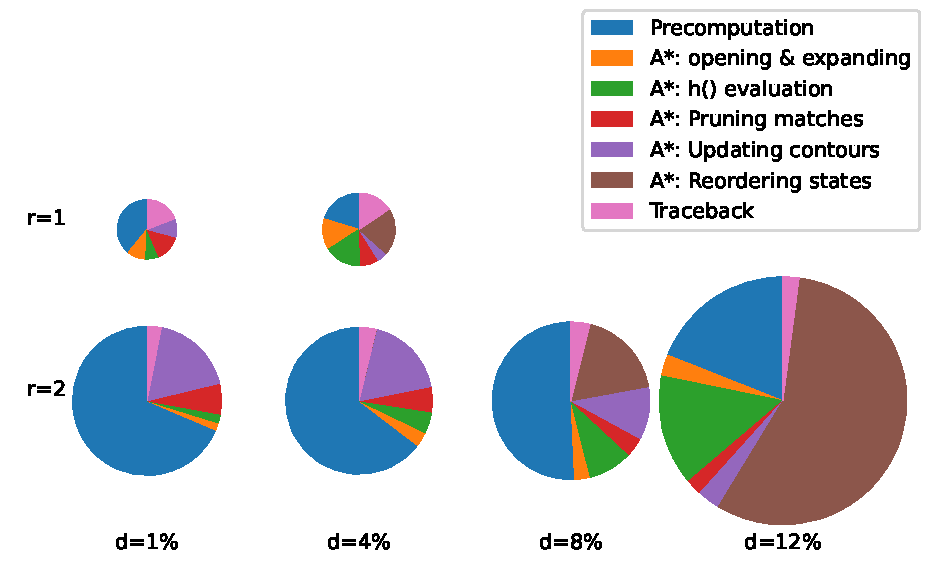
\includegraphics[scale=0.5]{plots/timing_synthetic.pdf}%
    \label{fig:timing-synthetic}
    }
    \subfloat[Human data]
    {
    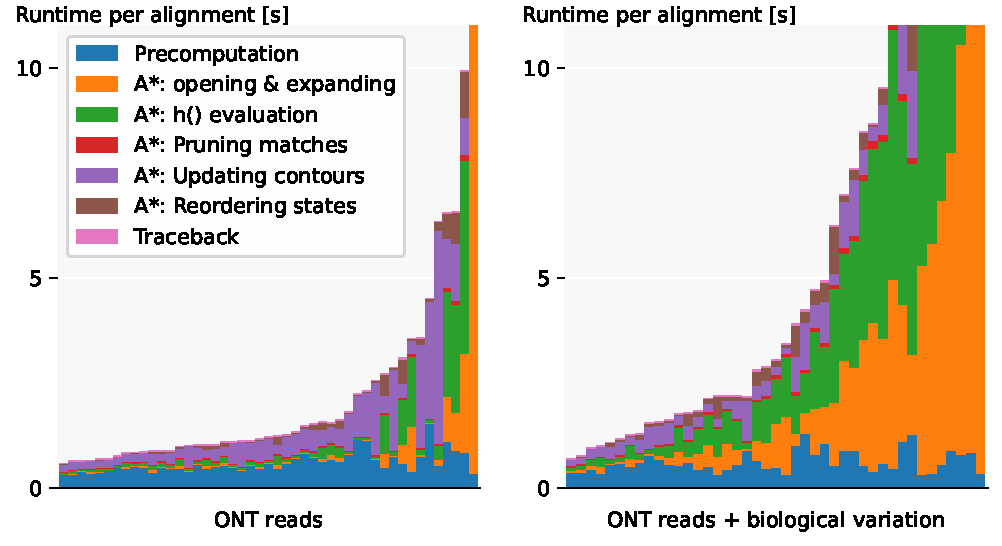
\includegraphics[scale=0.5]{plots/timing_real.pdf}%
    \label{fig:timing-human}
    } \caption[Runtime distributions per stage of \astarpa (\GCH with
    DT)]{\textbf{Runtime distributions per stage of \astarpa (\GCH with DT)}
    (stages do not overlap). Stage \emph{\A} includes expanding and opening
    states. \emph{Pruning matches} includes consistency checks. \emph{Updating
    contours} includes updating of contours after pruning.
    \protect\subref{fig:timing-synthetic} On synthetic data ($n{=}10^6\bp$,
    $N{=}10^7\bp$ total). The circle area is proportional to the total runtime.
    Figures for $r{=}1$ and $d{\geq}8\%$ are skipped due to timeouts
    ($\qty{100}{s}$). \protect\subref{fig:timing-human} On human data ($r{=}2$).
    Alignments are sorted by total runtime (timeouts not shown).}
\end{figure*}
